\textcolor{blue}{Problem 3}
Similar to problem $3$ in assignment $3$ and assignment $4$, you need to use the SUV dataset to implement (using Python or MATLAB) the $L_1$/$L_2$ regularization (penalty/augmented).
\begin{itemize}
    \item Present your code.
    \item Present the path plots of $L_1$ and $L_2$ regularization. (Notice: you need to mark the selected value of the regular parameter)
    \item Analyze the weight difference between $L_1$ and $L_2$ regularization. (Notice: you need to describe the similarities and differences between the solutions of path plots)
    \item If you only want to build a model that contains $2$ variables, which two features would you choose?
\end{itemize}

\textcolor{blue}{Solution}\\


1. The code and the method to run the code are all in the folder `code'.

2. The path plots of $L_1$ and $L_2$ regularization are shown in Figure \ref{fig:L1path} and Figure \ref{fig:L2path}.
Where the feature `Age' is seperate as: $0-20, 20-26, 26-30, 30-40, 40-50,$ others.\\
And feature `EstimatedSalary' is seperate as: $0-19500, 19500-40000, 40000-60000, 60000-80000, 80000-100000, 100000-130000, 130000-145000,$ others.\\
All features are normalize before training.\\

\begin{figure}[htbp]
    \center
    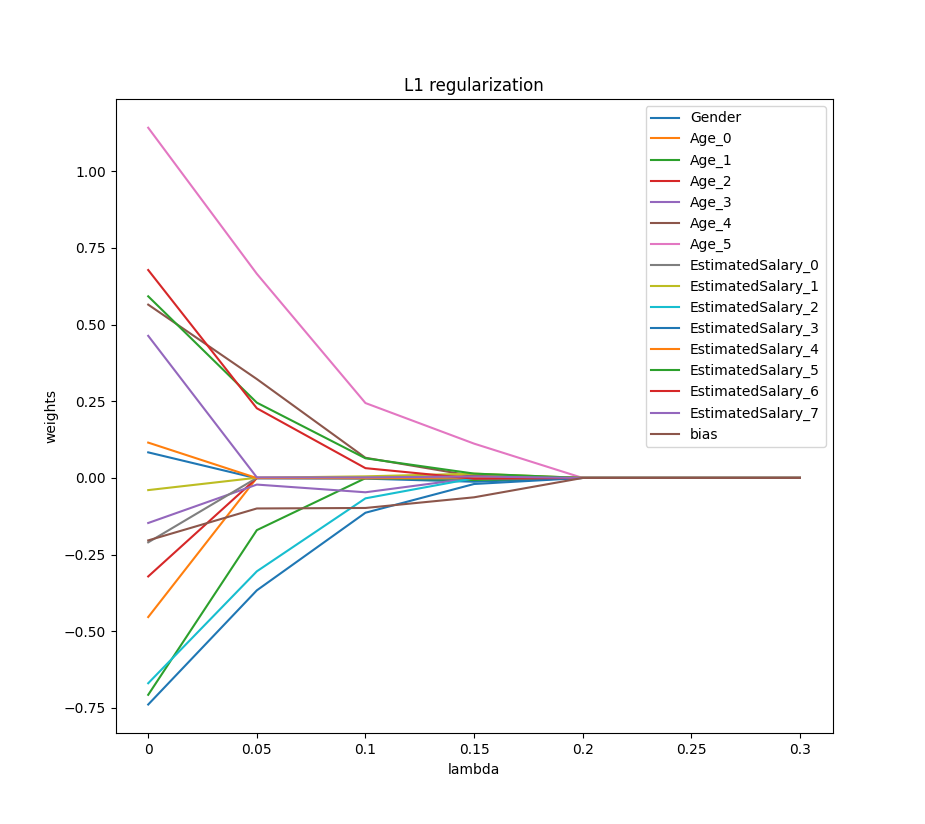
\includegraphics[width=\textwidth]{../fig/L1.png}
    \caption{Path plot of $L_1$ regularization}
    \label{fig:L1path}
\end{figure}

\begin{figure}[htbp]
    \center
    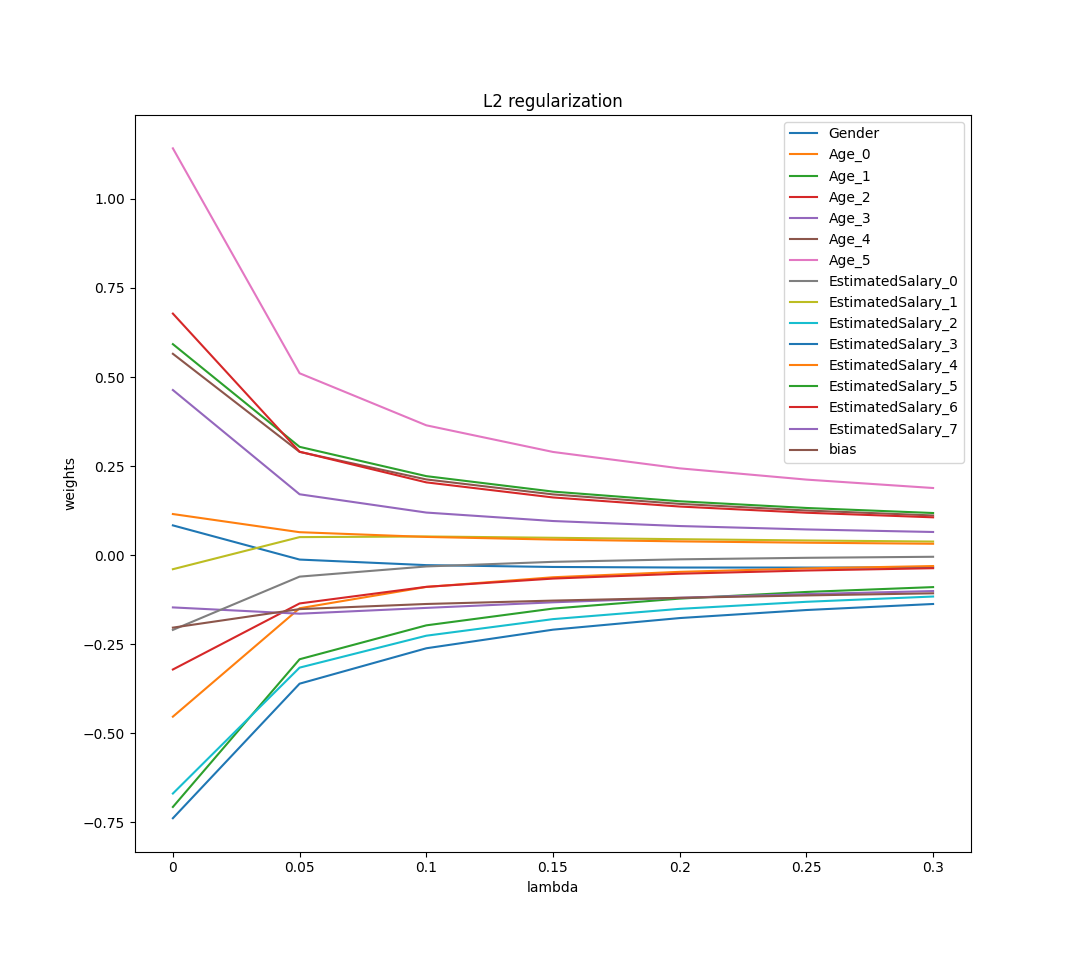
\includegraphics[width=\textwidth]{../fig/L2.png}
    \caption{Path plot of $L_2$ regularization}
    \label{fig:L2path}
\end{figure}

\ \\

3. We can see that both $L_1$ and $L_2$ regularization has the smaller weight as the regularization parameter $\lambda$ increases.
But the difference is that $L_1$ regularization can make some weights to be zero, which means that $L_1$ regularization can do feature selection.
But $L_2$ regularization can only make the weights smaller, but not zero.\\


4. If only want to build a model that contains $2$ variables,
For $L_1$ regularization, `Age\_5' and `bias' are chosen; for $L_2$ regularization, `Age\_5' and `EstimatedSalary\_3' are chosen.\\

This is because from the path plots, we can see that the weights of these two features have the largest absolute value when the regularization parameter $\lambda$ gets bigger.